\documentclass{bioinfo}

\usepackage{hyperref}
\usepackage{tikz}  
\usetikzlibrary{graphs}

\let\proglang=\textsf

\copyrightyear{2014}
\pubyear{2014}

\begin{document}
\firstpage{1}

\title[RDML]{RDML: an \textbf{R} Package for RDML Format Data Import}
\author[Sample \textit{et~al}]{Corresponding Author\,$^{1,*}$, Co-Author\,$^{2}$ and Co-Author\,$^2$\footnote{to whom correspondence should be addressed}}
\address{$^{1}$Department of XXXXXXX, Address XXXX etc.\\
$^{2}$Department of XXXXXXXX, Address XXXX etc.}

\history{Received on XXXXX; revised on XXXXX; accepted on XXXXX}

\editor{Associate Editor: XXXXXXX}

\maketitle

\begin{abstract}

\section{Motivation:}
One of the recommended elements in the Minimum Information for Publication of 
Quantitative Real-Time PCR Experiments (MIQE) guidelines is RDML file format. 
Despite the fact that the ability to export data in this format is implemented 
in software products of major PCR instruments, there is no tool allowing to work 
with the RDML format in R. 

\section{Results:}
We developed \textbf{R} package called RDML, which (i) reads fluorescence data obtained 
during qPCR and melting experiments and (ii) gets information about samples 
type, targets and concentration from RDML files generated by various PCR 
instruments; (iii) transforms fluorescence data to the appropriate format of the 
\textit{qpcR} and \textit{chiPCR} packages; (iv) generates human readable 
summary about all samples in experiment. 
\section{Availability:}
The \textbf{R} package RDML is implemented using R, and can be used in Windows, Mac, or 
Linux environments. It is available at CRAN and the latest version at 
https://github.com/kablag/RDML/.
\section{Contact:} \href{k.blag@yandex.ru}{k.blag@yandex.ru}
\end{abstract}

\section{Introduction}

Quantitative real-time PCR (qPCR) based on fluorescence detection is one the 
most popular methods in molecular biology, genetic, life science, agriculture 
and medicine disciplines. This method is fairly simple and at the same time 
provides accurate, reliable and reproducible 
information\cite{kubista_real-time_2006}. Second actively growing recently 
method with a fluorescence data using is a high-resolution melting 
\cite{reed_high-resolution_2007}\cite{wittwer_high-resolution_2009}

There are about twenty available real-time PCR cycler manufacturers, which in 
turn offers one or more models. Such a variety of models and manufacturers of 
both advantage and disadvantage. Users can select the appropriate models to them 
by number of samples at one run, the number of dyes, the method of work, the 
price and other parameters of the model. However, the majority of devices, even 
within a single manufacturer model range, using different methods of data 
processing and incompatible data storage formats. Applying different methods of 
data processing causes the PCR results obtained on different devices can not 
reliably be compared with results obtained by other devices. On the other hand, 
various storage formats do not allow to process the raw data from one instrument 
to another instrument software, and, more importantly, with the use of 
independent reference methods.

At this point, there is a document designed to allow comparison the results of 
qPCR and HRM analysis performed on different instruments -- MIQE guidelines 
\cite{bustin_miqe_2009, huggett_2013}. These guidelines suggest using the 
Real-time PCR Data Markup Language (RDML) as the main interchange format for PCR 
and HRM data. RDML promised to deliver a vendor independent and freely available 
file format, which is based on Extensible Markup Language (XML). Storage and 
exchange of qPCR data should be bidirectional. RDML data standard contains the 
the raw data acquired by the machine, sufficient information to understand the 
experimental setup (e.g., sample annotation, qPCR protocol, probe and primer 
sequences) and re-analyse the data and interpret the results 
\cite{lefever_rdml:_2009}. To the best of our knowledge is RDML  supported by 
Bio-Rad (CFX96 and CFX384), Life Technologies (StepOne, ViiA7, QuantStudio) and 
Roche (LC 2.0, LC96) thermo-cycler systems. Third party software (e.g., 
primer3plus \cite{untergasser_2007}, QPCR \cite{pabinger_2009}, LinRegPCR 
\cite{ruijter_2014}, \textit{qbase+} \cite{hellemans_2007}) are known to process 
the RDML-format. However, there is no implementation for the \textbf{R} language 
and environment for statistical computing and graphics. Thus, despite the 
presence of the open RDML format there is a lack in the software software 
capable of working with data in this format. Basically it is programs from 
manufacturers of PCR devices or commercial programs such as \textit{qbase+} 
\cite{rdml}. On the other hand, there are a number of open source processing 
solutions for PCR and melting curve analysis (e.g., HRM) 
\cite{roediger_RJ_2013,cousins_2012}, for example, implemented in \textbf{R} 
packages \textit{qpcR}\cite{ritz_qpcr:_2008} and \textit{chipPCR} 
\cite{roediger_chippcr_2014}.

The availability of an standard is also a prerequisite to many disciplines and 
can accelerate the advance in research. \textbf{R} has advanced internal 
capabilities to record of details about a particular analysis to easily 
recapitulate data from a study \cite{liu_2014}. The common approach for data 
management in \textbf{R} and \textbf{R} graphical user interfaces are native 
formats such as CSV, \textbf{R} workspaces as default data format or 
\cite{rodiger_rkward_2012, pabinger_2014, RDCT2014c}. However, a direct exchange 
with other systems was limited. An application of RDML is the distribution of 
data in an unified format. Though there are other approaches available in 
\textbf{R} for reproducible research \cite{Leeper_2014} we think is import to 
bridge the gab to other qPCR as recently reviewed in \cite{pabinger_2014}. in 
the advance of science \cite{gentleman_2004}. However, we argue that the 
\textit{RDML} package may serve as foundation for other \textbf{R} package 
hosted at Bioconductor \cite{gentleman_2004} and CRAN \cite{RCT}.

In this article we describe our \textbf{R} package \textit{RDML} which allows to 
import qPCR data from RDML~v1.1 format files and transform it to the human 
readable format appropriate to the \textit{qpcR} and \textit{chipPCR} packages. 
\textit{RDML} package is open-source, free to use, platform-independent, and 
thus can be modified for specific tasks or other \textbf{R} packages, even 
integrated to work-flows with other programming languages. Even though many qPCR 
instruments and software solutions are able work with the RDML format, there is 
a need make RDML available for the ever increasing used \textbf{R} environment.

\section{Implementation}

The most recent stable \textit{RDML} package is available at CRAN 
(\url{http://cran.r-project.org/web/packages/RDML/index.html}) and the 
developmental version is hosted at GitHub (\url{https://github.com/kablag/RDML}) 
with facilities to report bugs or request features. All package development 
followed the guidelines as descibed elsewhere \cite{RDCT2014a}. \textit{RDML} is 
implemented in \textbf{R}’s \emph{S3} class system. The naming convention in 
\textit{RDML} is \textit{lowerCamel} names \cite{Baaaath_2012}. Others and we 
support the opinion that data sets are an essential element of \textbf{R} 
packages for reproducible research 
\cite{gentleman_2004,hofmann_2013,Leeper_2014}. Therefore, we included XYZ data 
sets in the \textit{RDML} and the description of the experimental procedure. As 
of \textit{RDML} v.~0.4-2 we provide data sets from the Bio-Rad CFX 96, Roche 
LightCycler 2.0, Roche LightCycler 96 and Applied Biosystems StepOne.

Central functions of the \textit{RDML} package encompass the read-in of RDML 
data files and summary functions for RDML objects.

The RDML file format continues to develop coordinated by the RDML consortium 
(www.rdml.org/). Currently the improved RDML~1.1 version is used. Version~1.2 is 
currently being drafted. The \textit{RDML} package supports version~1.1.

Workflow of the \textit{RDML} function can be divided into five main stages (see Figure~\ref{fig:RDMLworkflow}):
\begin{itemize}
	\item \textbf{Unzip file} -- RDML file is a zip archive that contains one or more XML data files. Process of unzipping performs by built-in \textbf{R} function \textit{unzip}. Unzipped temporary file(s) deletes after ending of the next stage;
	\item \textbf{Parse inner XML tree} -- during this and next two stages we decided to use package \textit{XML} to parse XML tree and to get values from XML nodes;
	\item \textbf{Get general information} -- getting from XML such information as run targets, sample types, dilution series;
	\item \textbf{Get fluorescence data} -- forming from XML cycle/ fluorescence (for qPCR experiment) or temperature/ fluorescence (for melting experiment) tables and generating names by defined rules for each sample at run;
	\item \textbf{Combine into \textit{S3} class} -- combining of data obtained during previous stages into \textit{S3} class that represents \textit{list} of dilutions \textit{vector}, qPCR and/or melting data for samples in one table format or \textit{list} of tables spited by targets and samples types.
\end{itemize}

The \textit{RDML} package contains 3 data sets from Bio-Rad CFX 96, Life Technologies StepOne and Roche LightCycler 96 PCR machines.
\begin{figure*}
	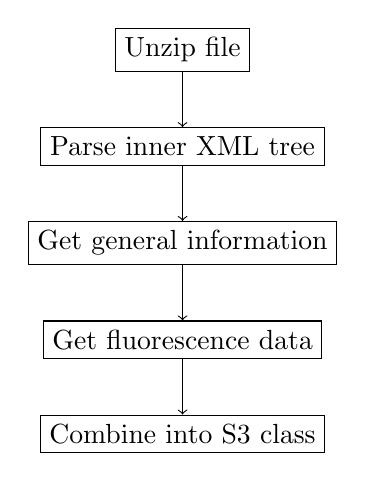
\begin{tikzpicture}
	\graph[nodes={align=center,rectangle,draw=black}, grow down sep=2em] {
		Unzip file -> Parse inner XML tree -> Get general information ->
		Get fluorescence data -> Combine into S3 class
	};
	\end{tikzpicture}
	\caption[]{\textit{RDML} workflow representation.}
	\label{fig:RDMLworkflow}
\end{figure*}

\begin{figure*}
\begin{verbatim}
# Use dataset lc96_bACTXY.rdml (in 'data' directory)
# generated by Roche LightCycler 96. Contains qPCR data
# with four targets and two types.
# Import with default settings.

PATH <- path.package("RDML")
filename <- paste(PATH, "/extdata/", "lc96_bACTXY.rdml", sep ="")
lc96 <- RDML(filename)

# Print the summary for the RDML object 'lc96'
summary(lc96)
\end{verbatim}
\end{figure*}


\section{Discussions and conclusions}

We developed \textit{RDML} package for \textbf{R} designed to provide user friendly fluorescence data import from RDML v1.1 format files. This package can be used as a part of the qPCR or HRM data processing workflows or for experiments overview.

\paragraph{Funding\textcolon}  Bio-Rad CFX 96 and Roche LightCycler 96 data sets were obtained at \textit{Center for collective use "Biotechnology"} of \textit{All-Russia Institute of Agricultural Biotechnology}.

%\bibliographystyle{natbib}
%\bibliographystyle{achemnat}
%\bibliographystyle{plainnat}
%\bibliographystyle{abbrv}
%\bibliographystyle{bioinformatics}
%
\bibliographystyle{plain}
%
\bibliography{RDML}

\end{document}
